\tikzset{every picture/.style={line width=0.75pt}} %set default line width to 0.75pt        

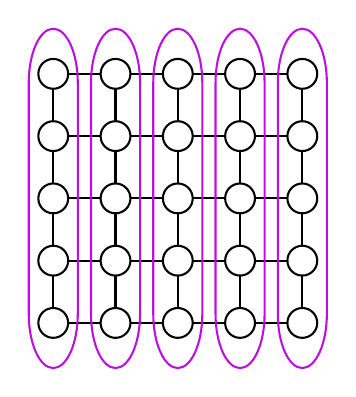
\begin{tikzpicture}[x=0.75pt,y=0.75pt,yscale=-1.5,xscale=1.5]
%uncomment if require: \path (0,130); %set diagram left start at 0, and has height of 130

%Shape: Grid [id:dp7399042803862277] 
\draw  [draw opacity=0][fill={rgb, 255:red, 255; green, 255; blue, 255 }  ,fill opacity=1 ] (369.5,25) -- (369.5,105.17) -- (289,105.17) -- (289,25) -- cycle ; \draw   (369.5,25) -- (289,25)(369.5,45) -- (289,45)(369.5,65) -- (289,65)(369.5,85) -- (289,85)(369.5,105) -- (289,105) ; \draw   (369.5,25) -- (369.5,105.17)(349.5,25) -- (349.5,105.17)(329.5,25) -- (329.5,105.17)(309.5,25) -- (309.5,105.17)(289.5,25) -- (289.5,105.17) ; \draw    ;
%Shape: Circle [id:dp8651637723303116] 
\draw  [fill={rgb, 255:red, 255; green, 255; blue, 255 }  ,fill opacity=1 ] (289.5,20.21) .. controls (292.15,20.21) and (294.29,22.35) .. (294.29,25) .. controls (294.29,27.65) and (292.15,29.79) .. (289.5,29.79) .. controls (286.85,29.79) and (284.71,27.65) .. (284.71,25) .. controls (284.71,22.35) and (286.85,20.21) .. (289.5,20.21) -- cycle ;
%Shape: Circle [id:dp9652078854977582] 
\draw  [fill={rgb, 255:red, 255; green, 255; blue, 255 }  ,fill opacity=1 ] (289.5,40.21) .. controls (292.15,40.21) and (294.29,42.35) .. (294.29,45) .. controls (294.29,47.65) and (292.15,49.79) .. (289.5,49.79) .. controls (286.85,49.79) and (284.71,47.65) .. (284.71,45) .. controls (284.71,42.35) and (286.85,40.21) .. (289.5,40.21) -- cycle ;
%Shape: Circle [id:dp1728749303967967] 
\draw  [fill={rgb, 255:red, 255; green, 255; blue, 255 }  ,fill opacity=1 ] (289.5,60.21) .. controls (292.15,60.21) and (294.29,62.35) .. (294.29,65) .. controls (294.29,67.65) and (292.15,69.79) .. (289.5,69.79) .. controls (286.85,69.79) and (284.71,67.65) .. (284.71,65) .. controls (284.71,62.35) and (286.85,60.21) .. (289.5,60.21) -- cycle ;
%Shape: Circle [id:dp23036347408038615] 
\draw  [fill={rgb, 255:red, 255; green, 255; blue, 255 }  ,fill opacity=1 ] (289.5,80.21) .. controls (292.15,80.21) and (294.29,82.35) .. (294.29,85) .. controls (294.29,87.65) and (292.15,89.79) .. (289.5,89.79) .. controls (286.85,89.79) and (284.71,87.65) .. (284.71,85) .. controls (284.71,82.35) and (286.85,80.21) .. (289.5,80.21) -- cycle ;
%Shape: Circle [id:dp44967083895831417] 
\draw  [fill={rgb, 255:red, 255; green, 255; blue, 255 }  ,fill opacity=1 ] (289.5,100.21) .. controls (292.15,100.21) and (294.29,102.35) .. (294.29,105) .. controls (294.29,107.65) and (292.15,109.79) .. (289.5,109.79) .. controls (286.85,109.79) and (284.71,107.65) .. (284.71,105) .. controls (284.71,102.35) and (286.85,100.21) .. (289.5,100.21) -- cycle ;
%Shape: Circle [id:dp9315039699787822] 
\draw  [fill={rgb, 255:red, 255; green, 255; blue, 255 }  ,fill opacity=1 ] (329.5,100.21) .. controls (332.15,100.21) and (334.29,102.35) .. (334.29,105) .. controls (334.29,107.65) and (332.15,109.79) .. (329.5,109.79) .. controls (326.85,109.79) and (324.71,107.65) .. (324.71,105) .. controls (324.71,102.35) and (326.85,100.21) .. (329.5,100.21) -- cycle ;
%Shape: Circle [id:dp5121103666957594] 
\draw  [fill={rgb, 255:red, 255; green, 255; blue, 255 }  ,fill opacity=1 ] (309.5,100.21) .. controls (312.15,100.21) and (314.29,102.35) .. (314.29,105) .. controls (314.29,107.65) and (312.15,109.79) .. (309.5,109.79) .. controls (306.85,109.79) and (304.71,107.65) .. (304.71,105) .. controls (304.71,102.35) and (306.85,100.21) .. (309.5,100.21) -- cycle ;
%Shape: Circle [id:dp4801713337694038] 
\draw  [fill={rgb, 255:red, 255; green, 255; blue, 255 }  ,fill opacity=1 ] (309.5,80.21) .. controls (312.15,80.21) and (314.29,82.35) .. (314.29,85) .. controls (314.29,87.65) and (312.15,89.79) .. (309.5,89.79) .. controls (306.85,89.79) and (304.71,87.65) .. (304.71,85) .. controls (304.71,82.35) and (306.85,80.21) .. (309.5,80.21) -- cycle ;
%Shape: Circle [id:dp12535689486360901] 
\draw  [fill={rgb, 255:red, 255; green, 255; blue, 255 }  ,fill opacity=1 ] (309.5,60.21) .. controls (312.15,60.21) and (314.29,62.35) .. (314.29,65) .. controls (314.29,67.65) and (312.15,69.79) .. (309.5,69.79) .. controls (306.85,69.79) and (304.71,67.65) .. (304.71,65) .. controls (304.71,62.35) and (306.85,60.21) .. (309.5,60.21) -- cycle ;
%Shape: Circle [id:dp46320678872772225] 
\draw  [fill={rgb, 255:red, 255; green, 255; blue, 255 }  ,fill opacity=1 ] (309.5,40.21) .. controls (312.15,40.21) and (314.29,42.35) .. (314.29,45) .. controls (314.29,47.65) and (312.15,49.79) .. (309.5,49.79) .. controls (306.85,49.79) and (304.71,47.65) .. (304.71,45) .. controls (304.71,42.35) and (306.85,40.21) .. (309.5,40.21) -- cycle ;
%Shape: Circle [id:dp6043516156300452] 
\draw  [fill={rgb, 255:red, 255; green, 255; blue, 255 }  ,fill opacity=1 ] (309.5,20.21) .. controls (312.15,20.21) and (314.29,22.35) .. (314.29,25) .. controls (314.29,27.65) and (312.15,29.79) .. (309.5,29.79) .. controls (306.85,29.79) and (304.71,27.65) .. (304.71,25) .. controls (304.71,22.35) and (306.85,20.21) .. (309.5,20.21) -- cycle ;
%Shape: Circle [id:dp6332387096370653] 
\draw  [fill={rgb, 255:red, 255; green, 255; blue, 255 }  ,fill opacity=1 ] (329.5,20.21) .. controls (332.15,20.21) and (334.29,22.35) .. (334.29,25) .. controls (334.29,27.65) and (332.15,29.79) .. (329.5,29.79) .. controls (326.85,29.79) and (324.71,27.65) .. (324.71,25) .. controls (324.71,22.35) and (326.85,20.21) .. (329.5,20.21) -- cycle ;
%Shape: Circle [id:dp055019880981398206] 
\draw  [fill={rgb, 255:red, 255; green, 255; blue, 255 }  ,fill opacity=1 ] (329.5,40.21) .. controls (332.15,40.21) and (334.29,42.35) .. (334.29,45) .. controls (334.29,47.65) and (332.15,49.79) .. (329.5,49.79) .. controls (326.85,49.79) and (324.71,47.65) .. (324.71,45) .. controls (324.71,42.35) and (326.85,40.21) .. (329.5,40.21) -- cycle ;
%Shape: Circle [id:dp8512639356233513] 
\draw  [fill={rgb, 255:red, 255; green, 255; blue, 255 }  ,fill opacity=1 ] (329.5,60.21) .. controls (332.15,60.21) and (334.29,62.35) .. (334.29,65) .. controls (334.29,67.65) and (332.15,69.79) .. (329.5,69.79) .. controls (326.85,69.79) and (324.71,67.65) .. (324.71,65) .. controls (324.71,62.35) and (326.85,60.21) .. (329.5,60.21) -- cycle ;
%Shape: Circle [id:dp6205062014645637] 
\draw  [fill={rgb, 255:red, 255; green, 255; blue, 255 }  ,fill opacity=1 ] (329.5,80.21) .. controls (332.15,80.21) and (334.29,82.35) .. (334.29,85) .. controls (334.29,87.65) and (332.15,89.79) .. (329.5,89.79) .. controls (326.85,89.79) and (324.71,87.65) .. (324.71,85) .. controls (324.71,82.35) and (326.85,80.21) .. (329.5,80.21) -- cycle ;
%Shape: Circle [id:dp222923337548673] 
\draw  [fill={rgb, 255:red, 255; green, 255; blue, 255 }  ,fill opacity=1 ] (349.5,20.21) .. controls (352.15,20.21) and (354.29,22.35) .. (354.29,25) .. controls (354.29,27.65) and (352.15,29.79) .. (349.5,29.79) .. controls (346.85,29.79) and (344.71,27.65) .. (344.71,25) .. controls (344.71,22.35) and (346.85,20.21) .. (349.5,20.21) -- cycle ;
%Shape: Circle [id:dp6018140604006843] 
\draw  [fill={rgb, 255:red, 255; green, 255; blue, 255 }  ,fill opacity=1 ] (349.5,40.21) .. controls (352.15,40.21) and (354.29,42.35) .. (354.29,45) .. controls (354.29,47.65) and (352.15,49.79) .. (349.5,49.79) .. controls (346.85,49.79) and (344.71,47.65) .. (344.71,45) .. controls (344.71,42.35) and (346.85,40.21) .. (349.5,40.21) -- cycle ;
%Shape: Circle [id:dp6348042495140271] 
\draw  [fill={rgb, 255:red, 255; green, 255; blue, 255 }  ,fill opacity=1 ] (349.5,60.21) .. controls (352.15,60.21) and (354.29,62.35) .. (354.29,65) .. controls (354.29,67.65) and (352.15,69.79) .. (349.5,69.79) .. controls (346.85,69.79) and (344.71,67.65) .. (344.71,65) .. controls (344.71,62.35) and (346.85,60.21) .. (349.5,60.21) -- cycle ;
%Shape: Circle [id:dp9647261865514132] 
\draw  [fill={rgb, 255:red, 255; green, 255; blue, 255 }  ,fill opacity=1 ] (349.5,80.21) .. controls (352.15,80.21) and (354.29,82.35) .. (354.29,85) .. controls (354.29,87.65) and (352.15,89.79) .. (349.5,89.79) .. controls (346.85,89.79) and (344.71,87.65) .. (344.71,85) .. controls (344.71,82.35) and (346.85,80.21) .. (349.5,80.21) -- cycle ;
%Shape: Circle [id:dp5724526378156161] 
\draw  [fill={rgb, 255:red, 255; green, 255; blue, 255 }  ,fill opacity=1 ] (349.5,100.21) .. controls (352.15,100.21) and (354.29,102.35) .. (354.29,105) .. controls (354.29,107.65) and (352.15,109.79) .. (349.5,109.79) .. controls (346.85,109.79) and (344.71,107.65) .. (344.71,105) .. controls (344.71,102.35) and (346.85,100.21) .. (349.5,100.21) -- cycle ;
%Shape: Circle [id:dp25061370635376257] 
\draw  [fill={rgb, 255:red, 255; green, 255; blue, 255 }  ,fill opacity=1 ] (369.5,20.21) .. controls (372.15,20.21) and (374.29,22.35) .. (374.29,25) .. controls (374.29,27.65) and (372.15,29.79) .. (369.5,29.79) .. controls (366.85,29.79) and (364.71,27.65) .. (364.71,25) .. controls (364.71,22.35) and (366.85,20.21) .. (369.5,20.21) -- cycle ;
%Shape: Circle [id:dp8340204987440425] 
\draw  [fill={rgb, 255:red, 255; green, 255; blue, 255 }  ,fill opacity=1 ] (369.5,40.21) .. controls (372.15,40.21) and (374.29,42.35) .. (374.29,45) .. controls (374.29,47.65) and (372.15,49.79) .. (369.5,49.79) .. controls (366.85,49.79) and (364.71,47.65) .. (364.71,45) .. controls (364.71,42.35) and (366.85,40.21) .. (369.5,40.21) -- cycle ;
%Shape: Circle [id:dp5677261375761635] 
\draw  [fill={rgb, 255:red, 255; green, 255; blue, 255 }  ,fill opacity=1 ] (369.5,60.21) .. controls (372.15,60.21) and (374.29,62.35) .. (374.29,65) .. controls (374.29,67.65) and (372.15,69.79) .. (369.5,69.79) .. controls (366.85,69.79) and (364.71,67.65) .. (364.71,65) .. controls (364.71,62.35) and (366.85,60.21) .. (369.5,60.21) -- cycle ;
%Shape: Circle [id:dp25189376094363247] 
\draw  [fill={rgb, 255:red, 255; green, 255; blue, 255 }  ,fill opacity=1 ] (369.5,80.21) .. controls (372.15,80.21) and (374.29,82.35) .. (374.29,85) .. controls (374.29,87.65) and (372.15,89.79) .. (369.5,89.79) .. controls (366.85,89.79) and (364.71,87.65) .. (364.71,85) .. controls (364.71,82.35) and (366.85,80.21) .. (369.5,80.21) -- cycle ;
%Shape: Circle [id:dp6141487714233882] 
\draw  [fill={rgb, 255:red, 255; green, 255; blue, 255 }  ,fill opacity=1 ] (369.5,100.21) .. controls (372.15,100.21) and (374.29,102.35) .. (374.29,105) .. controls (374.29,107.65) and (372.15,109.79) .. (369.5,109.79) .. controls (366.85,109.79) and (364.71,107.65) .. (364.71,105) .. controls (364.71,102.35) and (366.85,100.21) .. (369.5,100.21) -- cycle ;
%Flowchart: Terminator [id:dp5771267457316103] 
\draw  [color={rgb, 255:red, 189; green, 16; blue, 224 }  ,draw opacity=1 ] (297.38,27.94) -- (297.38,102.06) .. controls (297.38,111.69) and (293.85,119.5) .. (289.5,119.5) .. controls (285.15,119.5) and (281.62,111.69) .. (281.62,102.06) -- (281.62,27.94) .. controls (281.62,18.31) and (285.15,10.5) .. (289.5,10.5) .. controls (293.85,10.5) and (297.38,18.31) .. (297.38,27.94) -- cycle ;
%Flowchart: Terminator [id:dp1699164006075664] 
\draw  [color={rgb, 255:red, 189; green, 16; blue, 224 }  ,draw opacity=1 ] (317.38,27.94) -- (317.38,102.06) .. controls (317.38,111.69) and (313.85,119.5) .. (309.5,119.5) .. controls (305.15,119.5) and (301.62,111.69) .. (301.62,102.06) -- (301.62,27.94) .. controls (301.62,18.31) and (305.15,10.5) .. (309.5,10.5) .. controls (313.85,10.5) and (317.38,18.31) .. (317.38,27.94) -- cycle ;
%Flowchart: Terminator [id:dp4431975324978088] 
\draw  [color={rgb, 255:red, 189; green, 16; blue, 224 }  ,draw opacity=1 ] (337.38,27.94) -- (337.38,102.06) .. controls (337.38,111.69) and (333.85,119.5) .. (329.5,119.5) .. controls (325.15,119.5) and (321.62,111.69) .. (321.62,102.06) -- (321.62,27.94) .. controls (321.62,18.31) and (325.15,10.5) .. (329.5,10.5) .. controls (333.85,10.5) and (337.38,18.31) .. (337.38,27.94) -- cycle ;
%Flowchart: Terminator [id:dp948813775073037] 
\draw  [color={rgb, 255:red, 189; green, 16; blue, 224 }  ,draw opacity=1 ] (357.38,27.94) -- (357.38,102.06) .. controls (357.38,111.69) and (353.85,119.5) .. (349.5,119.5) .. controls (345.15,119.5) and (341.62,111.69) .. (341.62,102.06) -- (341.62,27.94) .. controls (341.62,18.31) and (345.15,10.5) .. (349.5,10.5) .. controls (353.85,10.5) and (357.38,18.31) .. (357.38,27.94) -- cycle ;
%Flowchart: Terminator [id:dp22652637896563754] 
\draw  [color={rgb, 255:red, 189; green, 16; blue, 224 }  ,draw opacity=1 ] (377.38,27.94) -- (377.38,102.06) .. controls (377.38,111.69) and (373.85,119.5) .. (369.5,119.5) .. controls (365.15,119.5) and (361.62,111.69) .. (361.62,102.06) -- (361.62,27.94) .. controls (361.62,18.31) and (365.15,10.5) .. (369.5,10.5) .. controls (373.85,10.5) and (377.38,18.31) .. (377.38,27.94) -- cycle ;
\end{tikzpicture}
